%======================================================================
\NEWSEC
%======================================================================

\subsection{\ssComponents}

%----------------------------------------------------------------------

\begin{frame}[fragile,label=ss-components] 
\secframetitle{\ssOop}
\framesubtitle{Cello software components}
\vspace{-0.2in}
\begin{center}
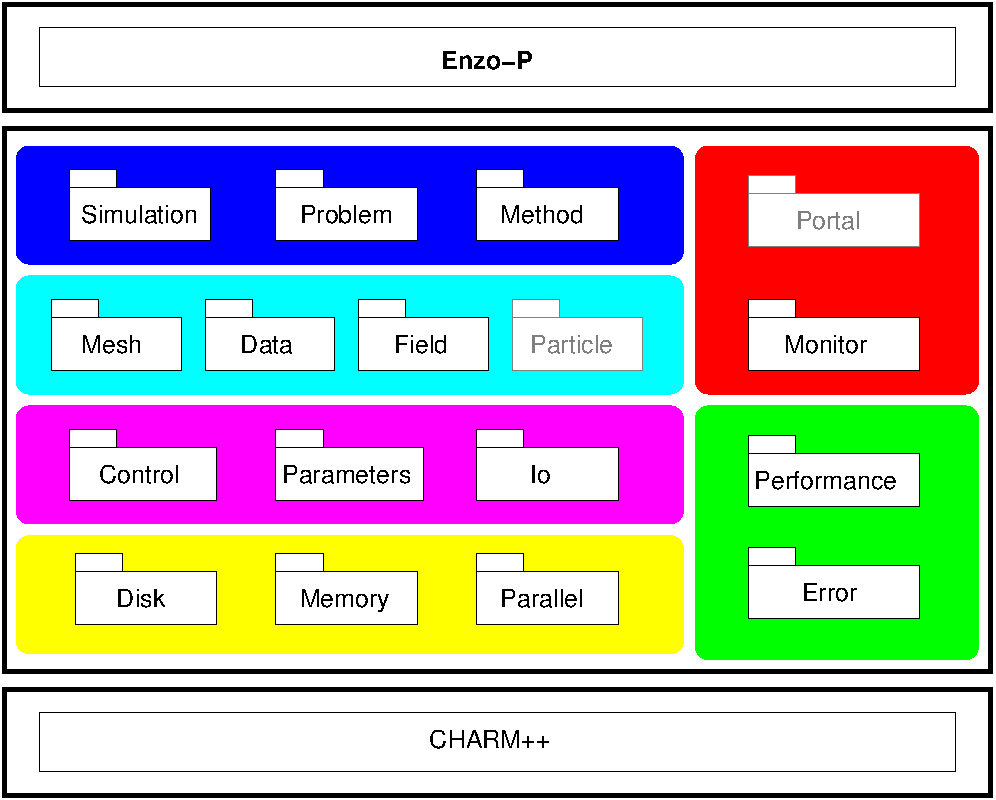
\includegraphics[width=3.0in]{components-1509.pdf}
\end{center}
\end{frame}

%----------------------------------------------------------------------

\begin{frame}[fragile] 
\secframetitle{\ssComponents}
\framesubtitle{Cello software components}
Cello's components are loosely grouped into categories
\begin{center}
\begin{minipage}{3in}
\begin{tabbing}
xxxxxxxxxxxxxxxxxxx\=\kill
\bluetext{High-level}\> \bluetext{Simulation}, \bluetext{Problem}, \bluetext{Method} \\
\cyantext{Data structures}\> \cyantext{Mesh}, \cyantext{Data}, \cyantext{Field}, \cyantext{(Particle)} \\
\magentatext{Middle-level}\> \magentatext{Control}, \magentatext{Parameters}, \magentatext{Io}  \\
\yellowtext{Hardware-interface}\> \yellowtext{Disk}, \yellowtext{Memory}, \yellowtext{Parallel} \\
\redtext{Interface}\> \redtext{Monitor}, \redtext{(Portal)}  \\
\greentext{Cross-cutting}\> \greentext{Performance}, \greentext{Error}
\end{tabbing}
\end{minipage}
\end{center}
\end{frame}

%----------------------------------------------------------------------

\begin{frame}[fragile] 
\secframetitle{\ssComponents}
\framesubtitle{\bluetext{High-level components}}
\bluebf{High-level components define the core classes in Enzo-P/Cello}

\begin{itemize}
\item \bluetext{Simulation}s define and manage computational \bluetext{Problem}s
(\bluecode{Simulation}, \bluecode{EnzoSimulation})
\item A \bluetext{Problem} defines the problem to be solved:
\begin{itemize}
\item numerical methods (\bluecode{EnzoMethodPpm}, etc.)
\item initial conditions (\bluecode{Initial})
\item boundary conditions (\bluecode{Boundary})
\item stopping criteria  (\bluecode{Stopping})
\item output (\bluecode{Output})
\item \textit{etc.}
\end{itemize}
\item A \bluetext{Method} implements a numerical method
\begin{itemize}
\item operates on block \bluetext{Data}
\end{itemize}

\end{itemize}
\end{frame}

%----------------------------------------------------------------------

\begin{frame}[fragile] 
\secframetitle{\ssComponents}
\framesubtitle{\cyantext{Data structure components}}
\cyanbf{Data structure classes define the AMR hierarchy and its data}

\begin{itemize}
\item \cyantext{Mesh} classes represent and operate on an AMR mesh (\cyancode{Hierarchy})
\item \cyantext{Data} classes store data on an AMR \textit{block} (\cyancode{Data}, \cyancode{EnzoData})
\item \cyantext{Field} classes store field data on a block
\begin{itemize}
\item \cyancode{FieldData}: field data on a block
\item \cyancode{FieldDescr}: global description of field data
\end{itemize}
\item \cyantext{Particle} classes will represent particle data on a block
\begin{itemize}
\item \cyancode{ParticleData}: particle data on a block
\item \cyancode{ParticleDescr}: global description of particle data
\end{itemize}
\end{itemize}
\end{frame}

%----------------------------------------------------------------------

\begin{frame}[fragile] 
\secframetitle{\ssComponents}
\framesubtitle{\magentatext{Middle-level components}}
\magentabf{Middle-level component interface high- and low-level classes}

\begin{itemize}
\item \magentatext{Control} handles problem evolution
\begin{itemize}
\item analagous to Enzo's \bluecode{EvolveHierarchy}, \bluecode{EvolveLevel}
\end{itemize}

\item \magentatext{Parameter} classes
\begin{itemize}
\item read parameters from a file (\magentacode{Parameters}) 
\item provide access to parameters (\magentacode{Config}, \magentacode{EnzoConfig})
\end{itemize}
\item \magentatext{Io} classes perform parallel IO
\begin{itemize}
\item \magentacode{OutputData} for writing data files
\item \magentacode{OutputImage} for writing image files
\item \magentacode{Schedule} for defining when to write files
\item \magentacode{IoHierarchy}, \magentacode{IoBlock}, \magentacode{IoFieldData}
interface data structure classes with \yellowtext{Disk} classes
\end{itemize}
\end{itemize}
%  include Control handles the time stepping of Method s to advance the
% problem forward in time, as well as sequencing adaptive mesh
% refinement data structure operations, including remeshing, scheduling
% dynamic load balancing (which will be delegated to Charm++), and
% refreshing ghost zones on Block boundaries. The Parameters component
% serves to read, store, and provide access to parameters defined in an
% input configuration file. To improve usability over Enzo,
% configuration files are more structured, and support floating-point
% and logical expressions to greatly simplify initializing problems with
% complex initial conditions. The Io component serves as a layer to
% coordinate the disk output of data structure components, such as
% Simulation Hierarchy and Field data. It calls the Disk component to
% handle actual file operations.  \end{frame}
\end{frame}

%----------------------------------------------------------------------

\begin{frame}[fragile] 
\secframetitle{\ssComponents}
\framesubtitle{\yellowtext{Hardware-interface components}}
\yellowbf{Hardware-interface components interface to system libraries}

\begin{itemize}
\item \yellowtext{Disk} classes write meta-data and data to files (\yellowcode{FileHdf5})
\item \yellowtext{Memory} tracks dynamic memory allocation
\item \yellowtext{Parallel} provides helper classes for parallelization
\begin{itemize}
\item \yellowcode{ArrayMap}: how to map chare array elements to processes
\item \yellowcode{Sync}: simple counter to ease Charm++ synchronization
\end{itemize}
\end{itemize}
% The lower-level components include Disk, Memory and Parallel. The Disk
% component implements basic disk operations, isolating the specific
% file format from the higher-level Io component. Disk currently
% supports HDF5, and we propose to support the Adaptable IO System
% (ADIOS) in the future to enhance transfer of data to and from other
% HPC software components. The Memory component controls dynamic memory
% allocation and management. Currently Memory handles allocating and
% monitoring heap memory usage; proposed functionality includes
% allocating, deallocating, and transferring data between main memory,
% hardware accelerator (GPU) memory, and many-core coprocessors
% (e.g.~the Intel Xeon Phi). As with the Disk component, this serves to
% isolate lower-level details from higher-level components. The Parallel
% component currently supplies basic access to core rank and core count,
% and is being depreciated.
\end{frame}

%----------------------------------------------------------------------

\begin{frame}[fragile] 
\secframetitle{\ssComponents}
\framesubtitle{\redtext{Interface} and \greentext{Cross-cutting} components}
\redbf{Interface components link Enzo-P / Cello with the outside world}

\begin{itemize}
\item \redtext{Monitor} keeps users informed of application status (\redcode{Monitor})
\item \redtext{(Portal)} will interface with external users / applications
\end{itemize}
\ \\
\ \\

\greenbf{Cross-cutting components are for globally-accessed classes}
\begin{itemize}
\item \greentext{Performance} measures and reports on application performance
\item \greentext{Error} provides basic error-handling support
\end{itemize}
% Interface compenents include Monitor (current) and Portal
% (proposed). The Monitor component controls the user-readable summary
% of progress to stdout, and the proposed Portal component will control
% the interaction of Enzo-P with external applications running
% concurrently, such as inline analysis or real-time visualization. One
% particular such analysis and visualization application is yt, which we
% will use to help drive the design and development of the Portal
% component.  
\end{frame}

%----------------------------------------------------------------------

%\begin{frame}[fragile] 
%\secframetitle{\ssComponents}
%\framesubtitle{: \greentext{Performance}, \greentext{Error}}
% Some Cello components can in principle be called from any software
% layer—these include Performance and Error. The Performance component
% dynamically collects performance data for the running Enzo-P
% simulation, and provides a holistic summary of performance data to the
% user, as well as to software components that can adapt to optimize
% desired performance metrics. Current metrics measured include memory
% usage (via the Memory component), and computation amount and memory
% access amount (via the Performance Application Programming Interface
% (PAPI). Future support will include metrics for monitoring parallel
% communication, dynamic load balancing, and disk usage. The Error
% component will be used to detect, evaluate, and decide what to do
% about software errors; higher-level error detection and recovery will
% be handled by Charm++, which supports both simple checkpoint to disk,
% as well as double in-memory checkpoint with automatic restart.
%\end{frame}


%    include component diagram (update from nsf proposal)
%    Go through each component and describe


%  Sequence diagram
%   Hardware components
%      Disk, Memory

% Mid-level-components

% Data structure components
%     Simulation
%     Hierarchy
%     CommBlock
%     Block
%     field\_block [field\_face]
%     [particle\_block]
%     example code

% Computational components

% Control components

% Cross-cutting components

%    Cello:     src/Cello/<component>\_<Class>.[hc]pp
%    Enzo-P:    src/Enzo/enzo\_<EnzoClass>.[hc]pp
%
%    examples
%
%    include Enzo component 
%
%    Note components are meant to be agile: can and have been redefined


% Top level components of Cello include . 
% 
% 
%Hardware-interface components
% 
%  Interface components
% 
%Cross-cutting components
% 


